Mammals -- and especially human beings -- are able to process diverse sensory input, learn and recognize complex spatial and temporal patterns, and generate behaviour based on context and previous experiences. While computers are efficient in carrying out numerical calculations, they fall short in solving cognitive tasks. Studying the brain and the neocortex in particular is an important step to develop new algorithms closing the gap between intelligent organisms and artificial systems. Numenta is a company dedicated to developing such algorithms and at the same time investigating the principles of the neocortex. Their \gls{htm} models are designed to solve real world problems based on neuroscience results and theories.

Efficiently simulating large-scale neural networks in software is still a challenge. The more biophysical details a model features, the more computational ressources are required. Different techniques for speeding up the execution of such implementations exist, e.g. by parallelizing calculations. Dedicated hardware platforms are also being developed. Digital neuromorphic hardware like the SpiNNaker platform often features highly parallelized processing architectures and optimized signal routing \citep{furber2014spinnaker}. On the other hand, analog systems directly emulate the neuron's behavior in electronic microcircuits. The \gls{hmf} is a mixed-signal platform developed in the scopes of the \gls{bss} and \gls{hbp}.

In this paper we present efforts in porting \gls{htm} networks to the \gls{hmf}. A framework for simulating \glspl{htm} based on spiking neural networks is introduced, as well as concrete network models for the spatial pooler and the temporal memory. The behavior of the latter is compared to software implementations in order to verify basic properties of the \gls{htm} networks. Having the features and limitations of the target platform in mind -- especially regarding synaptic plasticity --, we finally evaluate the applicability of the presented models.

\subsection{Hierarchical Temporal Memory}

\gls{htm} represents a set of concepts and algorithms for machine intelligence based on neocortical principles \citep{numenta2011htm}. It is designed to learn \emph{spatial as well as temporal patterns} and generate predictions from previously seen sequences. It features \emph{continuous learning} and operates on streaming data. An \gls{htm} network consists of one or multiple hierarchically arranged \emph{regions}. The latter contain neurons organized in columns. The functional principle is captured in two algorithms which are laid out in detail in the original whitepaper \citep{numenta2011htm}. The following paragraphs are intended as an introductory overview only and introduce the properties relevant to this work.

%\subsubsection{Spatial Pooler}
\label{sec:spatial_pooler_properties}

The \emph{spatial pooler} is designed to map a binary input vector to a set of
columns. By recognizing previously seen input data, it increases stability and
reduces the system's susceptibility for noise. Its behaviour can be
characterized by the following properties:

\begin{enumerate}
	\item\label{enm:spatial_pooler_sparsity} The columnar activity is sparse.
	Typically, 40 out of 2,048 colums are active, which is equivalent to a sparsity
	of \SI{2}{\%}. The number of active columns is constant in each time step and
	does not depend on the input sparsity.

	\item\label{enm:spatial_pooler_selection} The spatial pooler activates the $k$
	columns which receive the most input. In case of a tie between two columns, the
	active column is selected randomly, e.g. through structural advantages of
	certain cells compared to its neighbors.

	\item\label{enm:spatial_pooler_overlap} Stimuli with low pairwise overlap
	counts are mapped to sparse columnar representations with low pairwise
	overlap counts, while high overlaps are projected onto representations
	with high overlap. Thus, similar input vectors lead to a similar columnar
	activation, while disjunct stimuli activate distinct sets of cells.

	\item\label{enm:spatial_pooler_minimum} A column must receive a minimum input
	of e.g. 15 to become active.

\end{enumerate}

%\subsubsection{Temporal Memory}

The \emph{temporal memory} operates on single cells within columns and further
processes the spatial pooler's output. Temporal sequences are learned by the
network and can be used for generating predictions and highlighting anomalies.
Individual cells receive stimuli from other neurons on their distal dendrites.
This lateral input provides a temporal context. By modifying a cell's distal
connectivity, temporal sequences can be learned and predicted. The temporal
memory's behavior can be summarized by the following:

\begin{enumerate}

	\item Individual cells receive lateral input on their distal dendrites. In
	case a certain threshold is crossed, the cells enter a predictive
	(depolarized)state.

	\item\label{enm:temporal_memory_predictive} When a column becomes active due
	to proximal input, it activates only those cells that are in predictive state.

	\item\label{enm:temporal_memory_bursting} When a column with no predicted
	cells becomes active due to proximal input, all cells in a column burst. This
	phenomenon is referred to as \emph{columnar bursting}.

\end{enumerate}

\subsection{Heidelberg Neuromorphic Computing Platform}

The \gls{hmf} is a hybrid platform consisting of a traditional high-performance
cluster and a neuromorphic system. It is developed primarily at the
Kirchhoff-Institute for Physics in Heidelberg and the TU Dresden while receiving
funding from the \gls{bss} and \gls{hbp} \citep{hbp2014sp9spec}. The platform's
core is the wafer-scale integrated \gls{hicann} chip as shown in
Figure~\ref{fig:wafer}. Part of the chip's unique design is its mixed-signal
architecture featuring analog neuron circuits and a digital communication
infrastructure. Due to the short intrinsic time constants of the hardware
neurons, the system operates on an accelerated timescale with a speed-up factor
of \num{10e4} compared to biological real-time.

\begin{figure}
	\begin{center}
		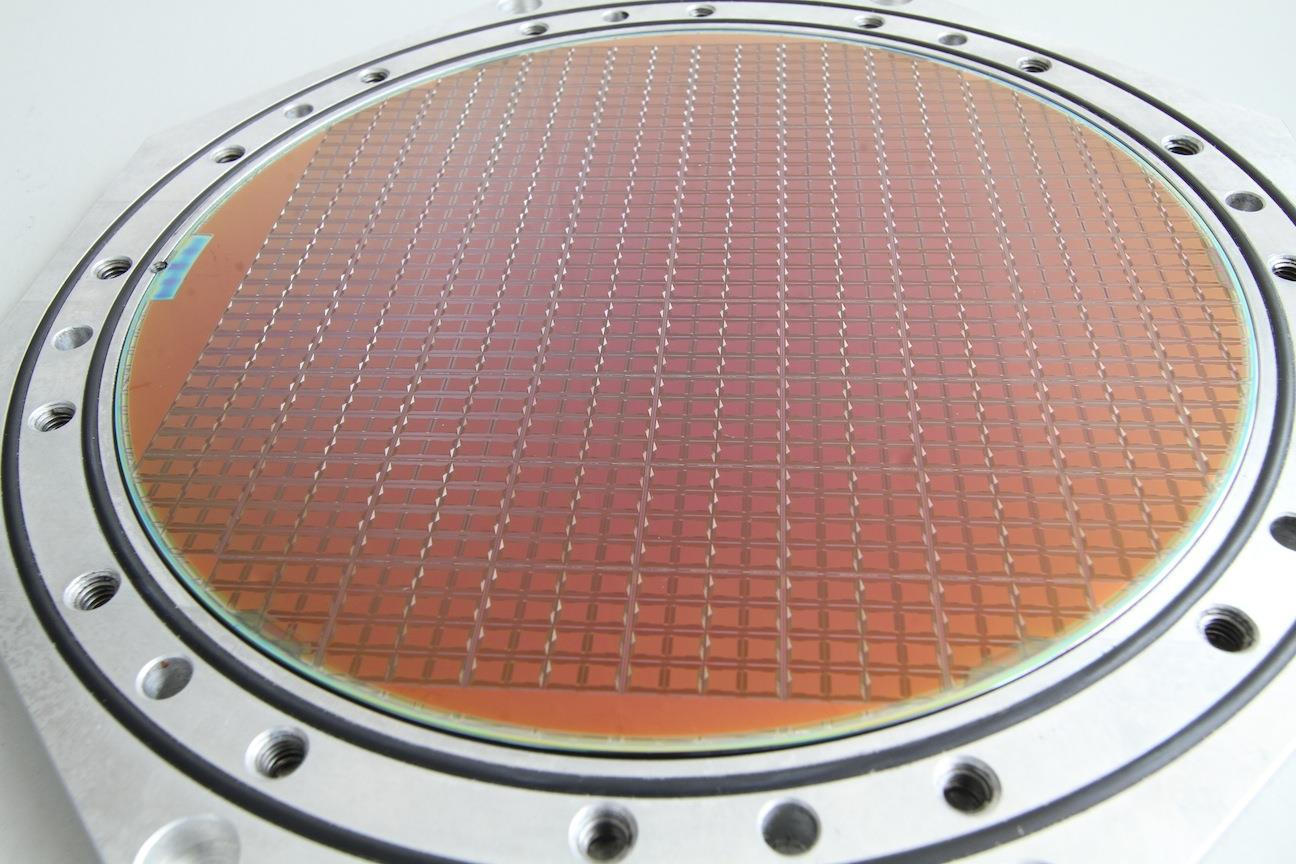
\includegraphics[width=\columnwidth]{assets/wafer.jpg}
	\end{center}
	\caption{A wafer containing 384 \gls{hicann} chips. The undiced wafer undergoes a custom post-processing step where additional metal layers are applied to establish inter-reticle connectivity and power distribution. (Photo courtesy of the Electronic Vision(s) group, Heidelberg.)}
	\label{fig:wafer}
\end{figure}

\gls{hicann} features 512 neurons (\emph{dendritic membrane circuits}). Each circuit can be stimulated via 226 synapses on two synaptic inputs. As a default, the latter are configured for excitatory and inhibitory stimuli, respectively. However, they can be set up to represent e.g. two excitatory inputs with different synaptic time constants or reversal potentials. By connecting multiple dendritic membranes larger neurons with up to \num{14e3} synapses can be formed.

A single wafer contains 384 chips with \num{200e3} neurons and \num{45e6} synapses. Multiple wafers can be connected to form even larger networks. The \gls{bss}'s infrastructure consists of six wafers and is being extended to 20 wafers for the first \gls{hbp} milestone.

%The \gls{hmf} is a mixed-signal neuromorphic platform developed at the Kirchhoff-Institute for Physics in Heidelberg and the TU Dresden. The project is funded within the \gls{bss} and the \gls{hbp}. Core of the system is the \gls{hicann} chip.
%
%\gls{hicann} features 512 analog point neurons -- or \emph{dendritic membranes} -- which can be stimulated via two independent synaptic inputs. As a default, the latter are configured for excitatory and inhibitory stimuli, respectively. However, they can be set up to represent e.g. two excitatory inputs with different synaptic time constants or reversal potentials. Multiple dendritic membrane circuits can be connected to form a larger neuron and allow for a higher number of synaptic inputs. Each dendritic membrane circuit can be stimulated via 113 synapses per synaptic input.
%
%The system's timescale results from the intrinsic time constants of the hardware neurons. The \gls{hmf} operates with a speed up of $10^4$ compared to biological real-time.

\subsection{Spiking Neuron Model}

There exist different techniques of varying complexity for simulating networks
of spiking neurons. The reference implementation we use for \gls{htm}  networks
is  based on first generation, binary neurons with discrete time steps
\citep{nupic}. Third generation models, however, incorporate the concept of
dynamic time and implement inter-neuron communication based individual spikes.

Starting from the original Hodgkin-Huxley equations \citep{Hodgkin1952},
multiple spiking neuron models were developed that feature different levels of
detail and abstraction. The \gls{hicann} chip implements \gls{adex} neurons
\citep{brette2005adaptive}. At its core, it represents a simple \gls{lif} model
but features a detailed spiking behavior as well as spike-triggered and
sub-threshold adaption. It was found to correctly predict approximately
\SI{96}{\%} of the spike times of a Hodgkin-Huxley-type model neuron and about
\SI{90}{\%} of the spikes recorded from a cortical neuron
\citep{jolivet2008quantitative}. On the \gls{hmf} and thus also in the following
simulations, the neurons are paired with conductance-based synapses allowing for
a fine-grained control of the synaptic currents and the implementation of e.g.
shunting inhibition.
